% Set page numbering to arabic the first time we commence a chapter.
% This is required to get the page numbering correct.
\pagenumbering{arabic}

% Note that the text in the [] brackets is the one that will
% appear in the table of contents, whilst the text in the {}
% brackets will appear in the main thesis.

%% CHAPTER HEADER /////////////////////////////////////////////////////////////////////////////////////
\chapter[Introduction]{Introduction}
\label{ch:intro}
The dissertation results from the author’s work as an assistant in the Department of Mechanics of Intelligent Structures, Institute of Fluid Flow Machinery, Polish Academy of Sciences.
Most of the work has been carried out within the framework of a research project titled ‘Model-assisted damage identification function for Structural Health Monitoring of composite structures under a varied environmental condition', which was granted to the author by the National Science Centre, Poland.
The primary objective was to develop a new approach to a sandwich structure assessment based on guided waves techniques under varied operating conditions.
The essence of the proposed method is to establish an accurate and numerically efficient model of the wave propagation in the sandwich structure to determine the severity of the damage.
A better understanding of guided wave behaviour in such structures and their interaction with damage will help develop more precise structural health monitoring strategies, reducing costs without compromising the safety of the liable systems.
%% CHAPTER INTRODUCTION ///////////////////////////////////////////////////////////////////////////////

%% INCLUDE SECTIONS ///////////////////////////////////////////////////////////////////////////////////
%% SECTION HEADER /////////////////////////////////////////////////////////////////////////////////////
\section{Sandwich Composite Structures}
\label{sec:scs}

%% SECTION CONTENT ////////////////////////////////////////////////////////////////////////////////////
Composites consist of two or more different materials, such as plastics, resins, metal alloys, glass, carbon or bio-based fibres. The combination of material constituents gives  structure benefits from the properties of the component materials, e.g., the strength of carbon fibres and the low density of the polymer resin in the case of \ac{cfrp}.
The contribution of lightweight composite materials to the production of structural components has been increasing rapidly since the middle of the last century.
Due to the high strength-to-weight ratio, higher operating temperatures, greater stiffness and higher
reliability, composite materials are extensively used in the aircraft and aerospace industry and civil constructions.
Composites account for more than 50\% of the total weight of the aircraft Boeing B787 and Airbus A350 \cite{giurgiutiu2015structural}.

One group of composites includes sandwich panels, which is a type of multi-layered structure that are composed of the mid-core sandwiched between thin skins.
The skins, made of high strength materials, are designed to carry tensile or compressive stresses from longitudinal forces and bending moments.
On the other hand, the core transmits mainly shear stresses from transverse forces.
It also separates the skins, which increases structural stiffness for thin layers, improves insulation properties, and reduces weight while maintaining strength properties similar to the solid construction of the same density.
A popular core used in engineering structures is a honeycomb geometry core.
Fig.~\ref{fig:hcp} shows the construction of the \ac{hsc}.
The core can be made of aluminium, cardboard or Nomex. 
\begin{figure}[H] %hbtp
	\begin{center}
		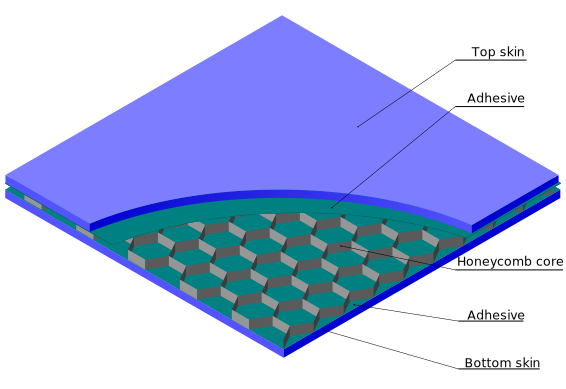
\includegraphics{Intro/honeycomb_plate}
		\caption{
			\label{fig:hcp} Structure of the honeycomb sandwich composite.}
		\vspace{-0.5cm}
	\end{center}
\end{figure}

However, these complex structures are exposed to various types of damage that are not found in metal alloy materials, e.g., hidden disbonds between the skin and the core, delamination of the composite skins, or the core impact damage.
They can occur either during a manufacturing process, storage or in-service life.
Therefore, advanced methods are required for online damage detection.
Thus, the use of composites has forced the development of advanced approaches to structural inspections, e.g., methods based on elastic wave propagation had to account for the anisotropic structure of the material.
%% SECTION HEADER /////////////////////////////////////////////////////////////////////////////////////
\section{Structural health monitoring}
\label{sec:scm}

%% SECTION CONTENT ////////////////////////////////////////////////////////////////////////////////////
\Ac{shm} is the process of implementing an advanced damage identification strategy for structural or mechanical systems \cite{farrar2007introduction}.
The \ac{shm} systems usually consist of a sensor network, a \ac{dau}, and a central processor.
The \ac{dau} is responsible for collecting the data measured by the sensor network.
A central unit then determines the current state of the structure through signal processing and statistical classification.
The implementation of \ac{shm} aims to extend the safe life of the monitored system, or usage of lightweight materials, which leads to cost reduction in production and operation.
For example, composites and adhesive bonding techniques reduces the aircraft's overall weight, reducing fuel consumption \cite{scelsi2011potential}.
\ac{shm} is most commonly found in structures, such as aerospace, civil and mechanical engineering, where damage can have catastrophic consequences.

Rytter, in his dissertation \cite{rytter1993vibrational}, classified the \ac{shm} system advancement into the following four levels:
\begin{itemize}
	\item[] \textbf{Level 1}: Detection.
	\item[] \textbf{Level 2}: Localization.
	\item[] \textbf{Level 3}: Assessment.
	\item[] \textbf{Level 4}: Consequence.
\end{itemize}
The first level determines if any adverse change in the geometric has occurred or material characteristics of the system. The second level leads to the localization of the damage.
The third and fourth level systems determine the size of the flaw and decide whether any maintenance is necessary, respectively.
The existence and location of faults can be defined in unsupervised learning mode by taking a threshold value for a measurable, damage-sensitive system feature. The threshold should be compensated depending on the prevailing operational and environmental conditions.
In contrast, damage size is determined in supervised learning mode based on an analytical model or data extracted experimentally from the structure \cite{worden2007fundamental}.
%% SECTION HEADER /////////////////////////////////////////////////////////////////////////////////////
\section{Piezoelectric Transducers}
\label{sec:challenges}

%% SECTION CONTENT ////////////////////////////////////////////////////////////////////////////////////


%% SECTION HEADER /////////////////////////////////////////////////////////////////////////////////////
\section{Chosen \ac{shm} techniques using \acp{pzt}}
\label{sec:techniques}

%% SECTION CONTENT ////////////////////////////////////////////////////////////////////////////////////

\subsection{Guided waves based techniques}


\Acp{gw} are mechanical vibrations being a superposition of shear and longitudinal waves propagating in a bounded elastic medium, e.g., bars, beams, rods, plates and shells. 
Guided waves are multi-modal and dispersive, i.e. more than one mode travels simultaneously through the medium with the phase velocity depending on the frequency.
Fig.~\ref{fig:dispersion} shows an example of dispersion curves generated by the Dispersion Calculator~\cite{huber2021dispersion} software tool for a 1 mm thick \ac{cfrp} plate in the frequency range 0-2000 kHz.
\Ac{a0} and \ac{s0}, considering the distribution of particle displacements on the upper and lower free surface relative to a central surface, are observed for low frequencies.
The mode shapes are pictured in Fig.~\ref{fig:mode_shape}, with the \ac{s0} particle displacements being dominant in-plane, while the \ac{a0} is dominated by out-of-plane.
Moreover, higher harmonic modes appear over the cut-off frequency, as shown in Fig.~\ref{fig:dispersion}.
\begin{figure}
	%	\begin{center}
	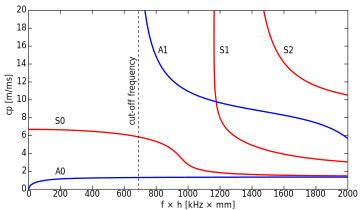
\includegraphics[width=1\linewidth]{Intro/dispersion}
	%	\end{center}
	\caption{Dispersion diagram for a 1 mm \ac{cfrp} plate (adopted from Dispersion Calculator~\cite{huber2021dispersion}). Red and blue solid curves represent symmetric and antisymmetric modes, respectively; a black dashed line indicates the cut-off frequency for higher modes.}
	\label{fig:dispersion}
\end{figure}
\begin{figure}
	%	\begin{center}
	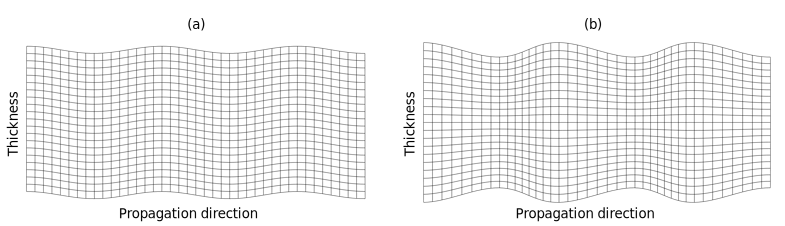
\includegraphics[width=1\linewidth]{Intro/mode_shape}
	%	\end{center}
	\caption{Mode shape of the \textbf{(a)} \ac{a0} and \textbf{(b)} \ac{s0} at 100 kHz for \(\phi=0^{\circ}\) in 2 mm composite plate (exported from Dispersion Calculator~\cite{huber2021dispersion}).}
	\label{fig:mode_shape}
\end{figure}

Detection schemes based on \acp{gw} exploit reflection, attenuation, and mode conversion when the propagating wave encounters a discontinuity in the structure \cite{alleyne1992interaction}.
Thus, this technique is efficient in detecting various types of defects, such as delamination \cite{sohn2011delamination,tian2015delamination}, adhesive disbonds \cite{rucka2018damage,balasubramaniam2021ultrasonic}, corrosion changes \cite{alleyne1995long,lowe1998defect}, cracks \cite{tua2004detection,lu2006crack,zima2020detection} and failures occurring in \acp{hsc} \cite{mustapha2011assessment, sikdar2016guided, sikdar2016ultrasonic,radzienski2016assessment, yu2019core}.
Many techniques based on \ac{gw} propagation have been developed for damage detection and localization.
A pitch-catch technique \cite{ihn2008pitch, sikdar2017structural} uses a pair of detached sensors, one excites, and the other receives a signal.
If the wave encounters a defect between the sensors, it will scatter, and the recorded signal will be distorted.
In the case of the pulse-echo technique \cite{guo1993interaction, kudela2008damage}, there is one sensor that excites the wave and, at the same time, registers possible echoes from the damage.
The damage localization can be determined if the wave speed is known and the time of flight is measured.
The radar principles were utilized in a phased array technique for plate inspection \cite{giurgiutiu2004embedded, ostachowicz2008elastic, kudela2018structural}.
The technique uses an array of transducers, each excited with an appropriate time offset, to focus all the waves at a single grid point of the area to be inspected.
A damage map is determined once the signals are obtained and processed for the entire grid.
Fink proposed a different approach, developing what he called a time-reversal mirror \cite{fink1992time}.
In this method, the wave propagates from one sensor to another, and then after time-reversal and dispersion compensation, the wave is re-emitted to the origin sensor.
The resulting signal will be a mirror image of the forcing signal only if the wave does not encounter damage along the way \cite{park2007time, eremin2016analytically}.

The \acp{pzt} can be used mutually as actuator-receiver pairs or as a single actuator with other types of devices, e.g. \ac{sldv}, \ac{fbg} sensors.
The \acp{pzt} generate high forces with broadband frequency, so methods based on \ac{gw} can detect various damage types of different sizes in a large inspected area.
Moreover, specific algorithms do not require a baseline model, and the method implementation is economically efficient.

\subsection{Electromechanical impedance methods}
\Ac{emi} spectroscopy is also an effective and powerful technique in \ac{shm} for real-time structural damage assessment \cite{park2003overview}.
The basis of this method is the influence of the mechanical impedance of the inspected host structure on the electrical impedance of the \ac{pzt} attached to the structure.
Assuming that the mechanical property of the sensor remains unchanged over the monitoring period, any changes in measurements of the electrical impedance can be considered a difference in the structure stiffness, which in turn can indicate that a defect has occurred.

Fundamentals of the \ac{emi} method were introduced by Liang et al. \cite{liang1994impedance}.
An analytical model of a \ac{pzt} actuator bonded to one end of a single degree of freedom mass-spring-damper system was presented in this pioneering work.
In the early papers, the authors adopted quasi-static sensor approximation until  Giurgiutiu and Zagrai \cite{giurgiutiu2000characterization} derived an expression where the sensor dynamic was incorporated.
The dynamics of a single \ac{pzt} with various boundary conditions (free, clamped and elastically constrained) and sensor attached to a beam were considered.
Further investigation was performed for the sensor bonded to the host structures was performed \cite{zagrai2001electro, giurgiutiu2005damage}.
Damage detection is realized by comparing the state of the structure with the reference state using overall statistical damage indices, e.g., the \ac{rmsd}, the \ac{mapd}, \ac{ccd} and \ac{pnn}.
Malinowski et al. \cite{malinowski2014characterisation, malinowski2015use} investigated the effects of \ac{emi} changes related to the state of the adhesive layer between two composite plates.
The technique has been used to evaluate weak bonds due to inadequate adhesive curing temperature, release agent and moisture contamination. This type of damage is not detectable using the method based on \ac{gw} propagation.
Experimental testing was conducted on weakened samples and compared with a reference.
The \ac{rms} of the conductance in the range of 3-5 MHz and the first thickness resonant frequency shift were considered for bond-line assessment.

An and Sohn \cite{an2012integrated} proposed a new damage detection technique that combines \ac{emi} and \ac{gw} advantages.
In the method, measured admittance characteristic is separated into two parts: active and passive.
\Ac{di} is a weighted sum of two indicators obtained from \ac{gw} signal and active admittance.
Because passive impedance is only sensitive to temperature variation, it is used for temperature compensation on both mentioned signals.
Instead of two \acp{di}, Sevillano et al. \cite{sevillano2016damage} proposed more integrated \ac{di} based on the electromechanical power dissipation of the \ac{pzt} sensor.

The \ac{emi} technique can detect damage, such as delamination or cracks, but is also sensitive to changes, such as weak bonds, which the \ac{gw} method is ineffective at detecting.
However, the \ac{emi} is a local method for the high frequency.
Giurgiutiu et al. \cite{giurgiutiu2001electro} obtained consistent results for crack detection in distances up to 40 mm in the frequency range 300-450 kHz. 
This method is also sensitive to environmental conditions such as temperature and humidity fluctuations\cite{bhalla2002practical} or loading variations \cite{lim2011impedance}.

%\subsection{Modal analysis techniques}
%% SECTION HEADER /////////////////////////////////////////////////////////////////////////////////////
\section{Challenges in \acs{gw} propagation modelling for damage assessment in the \acs{hsc}}
\label{sec:challenges}

%% SECTION CONTENT ////////////////////////////////////////////////////////////////////////////////////
The assessment of the damage severity in structural materials requires the development of a database of the effect of damage on system response \cite{worden2007fundamental}.
In the case of the \ac{hsc}, many factors affect the \ac{di} magnitude, such as damage localisation, material properties and dimensions, the sensor position relative to the core cell and the boundary conditions.
Considering all the factors, the determination of DI by experimental means becomes very complicated, expensive and time-consuming.
Therefore, numerical analysis and computer simulations become the only practical tool to achieve the goal.

The most common \ac{hsc} numerical model used in analysing \acp{gw} and \ac{emi} found in the literature is the model based on the \ac{fem}.
Although the numerical results are close to the experimental results, the models have some limitations in performing the simulations in a reasonable computation time and operating memory consumption.
In order to alleviate these limitations the following techniques are employed:
\begin{itemize}
\item reduction of the sample dimensions \cite{hosseini2013numerical, tian2015wavenumber};
\item homogenisation of the core properties \cite{catapano2014multi, zhou2020debonding};
\item a simplified \ac{2d} model based on a cross-section of the panel \cite{li2019detection};
\item omission of an adhesive layer \cite{mustapha2013non}.
\end{itemize}

The time and memory consumption of the \ac{fem} simulations is due to the high spatial resolution needed to converge the numerical results.
When first-order elements are used, up to 20 nodes per the shortest wavelength of interest is recommended by Moser et al. \cite{moser1999modeling}.
At a time when the operational capabilities of personal computers were severely limited, several methods derived from classic \ac{fem}, were developed to increase the efficiency of calculations. 
The \ac{bem} has been widely used for wave propagation in infinite or semi-infinite areas \cite{brebbia1984boundary}.
This method uses the fundamental solution of a \ac{pde} with the approximation only at the boundary of the domain.
The \ac{fdm} also has found application in the elastic waves modelling \cite{delsantoO1992connection}. 
Solution of the \ac{pde} is realised by the Taylor expansion with the arbitrary number of terms that determines the order of accuracy \cite{willberg2015simulation}.
The main disadvantage of this method is the loss of numerical stability for the structure with varying material properties.

To avoid this drawback, Delsanto et. al developed the \ac{lisa} with the combination of sharp interface model to connect to different domains \cite{delsantoO1992connection}. This method is the extension of the \ac{fdm} in which iteration equations are obtain directly from heuristic consideration \cite{willberg2015simulation}.
The \ac{lisa} is highly numerical effective due to local interactions between elements are directly transferred for numerical calculations.
Additional, the method is available to parallel computations on \ac{gpu} \cite{packo2012lamb}.

However, no application of the \ac{bem}, \ac{fdm} and \ac{lisa} in the HSC modeling has been found in the literature.
To implement complex core geometries while maintaining numerical efficiency, a method based on higher-order elements can be a good solution.
The implementations of this technique have been developed in recent years, achieving convergence even at six nodes \cite{willberg2012comparison}.
One is a method based on Lagrange polynomials as a shape function and \ac{gll} for integration scheme, termed \ac{sem}.
The \ac{sem} was initially developed for the numerical solution of the fluid flow in a channel by Patera \cite{patera1984spectral}.
The method has also been successfully employed for acoustic wave propagation in geological structures \cite{seriani1994spectral, komatitsch2000simulation},  and \ac{gw} propagation in engineering elements \cite{kudela2007wave, ostachowicz2011guided, rucka2010experimental,rekatsinas2017cubic}.
The time-domain \ac{sem} can be applied to complex structures e.g. stiffened panels \cite{schulte2011simulation, lonkar2014modeling}.
Versatility of the method is also related to the use of hybrid elements in combination with \ac{fem} formulation \cite{ha2009optimizing} and non-linear issues \cite{yu2020time, li2021hybrid}.

Due to the fast convergence and flexibility of the \ac{sem}, Kudela \cite{kudela2016parallel} applied the method to the \ac{hsc} model with the \ac{fcgm}.
However, the author used \ac{3d} elements to model the core walls resulting in a huge number of \acp{dof}.
The model size could be reduced if the shell element replaced the solid one.
In addition, the surface-mounted \ac{pzt} is omitted in the above model, and a concentrated force is used as the disturbance source.
The sensors mesh would have to coincide with the plate mesh or use the coupling between both meshes to include the \acp{pzt} in the simulation.
Such coupling can be realised using an interface based on Lagrange multipliers proposed by Farhat and Roux for domain decomposition in \ac{fem} \cite{farhat1991method}.
Ashwin et al. implemented the interface for the \ac{sem} but did not adopt it to non-matching grids \cite{ashwin2014formulation}, which is required for model generalization.
My aim was to implement non-matching grid approach for the \ac{sem} and also enable coupling between shell and \ac{3d} elements.

The efficient model and the computational hardware play a significant role in the simulation speed. 
Kudela presented the \ac{sem} algorithm for parallel calculation on the \ac{gpu} \cite{kudela2016parallel}.
The multi-core architecture of the \ac{gpu} enables simultaneous vector operations, making simulations over 14 times as fast as those performed by a \ac{cpu}.
Therefore, using the \ac{gpu} card will make it more convenient to perform simulations of models with large number of \acp{dof} to determine the effect of damage size on system response.
Thus, the time integration algorithm must be modified to make parallel computing on the GPU still possible despite the usage of interface elements.


\section{Conclusions}
\label{sec:conclusionsIntro}

%% SECTION CONTENT ////////////////////////////////////////////////////////////////////////////////////
In the Introduction, a brief overview of problems undertaken in the dissertation has been presented, i.e., composite materials, construction and their applications;  definition of the \ac{shm} and application of \ac{pzt} sensors in damage detection; and challenges in \ac{gw} propagation modelling for damage severity assessment in the \acp{hsc}.
The most relevant issues address to:
\begin{itemize}
	\item flexibility to model complex structure of the honeycomb core;
	\item time efficiency due to the high number of \ac{dof} of the model;
	\item possibility to parallel calculation on the \ac{gpu}.
\end{itemize}
The literature review revealed the need for a practical tool for damage size estimation in the \acp{hsc} to increase the safe usage of the engineering structures made of composites. 
Therefore, in the dissertation, I have tried to develop an effective way to determine the function of the effect of damage size on elastic wave propagation.
